\section*{Overview - Bachelor's thesis }

\subsection*{Cell models}

Definitions of continuous \textbf{Centre Radius Form (CRF)}:

\begin{definition} \textbf{Centre radius form (CRF)} \label{def:CRF}  \\
	For a given point $\vec{c} \in \mathbb{R}^2$ and function $r: [0, 2\pi) \rightarrow (0, \infty)$ so that $r \in C^1([0, 2\pi))$, $r(0) = r(2\pi)$ and $r'(0) = r'(2\pi)$, the tuple $(\vec{c}, r)$ describes a cell in its centre radius form (CRF) with centre point $\vec{c}$ and radius $r(\phi)$ at angle $\phi \in [0, 2\pi)$ that is taken with the $x$ axis. \\
\end{definition}

and \textbf{Discrete Form (DF)}:

\begin{definition} \textbf{Discrete form (DF)} \label{def:DF}  \\
	An ordered sequence of points $C = (\vec{x}_1, \ldots , \vec{x}_N)$ is considered to be a cell in its discrete form (DF) if the polygon that results when connecting every point with its neighbours and $\vec{x}_1$ with $\vec{x}_N$ is simple and positively orientated. \\	
	Cells in the DF model are sometimes just called discrete cells. \\
\end{definition}

\begin{figure}[b!]
	\centering
	\hfill
	\begin{subfigure}{0.4\textwidth}
		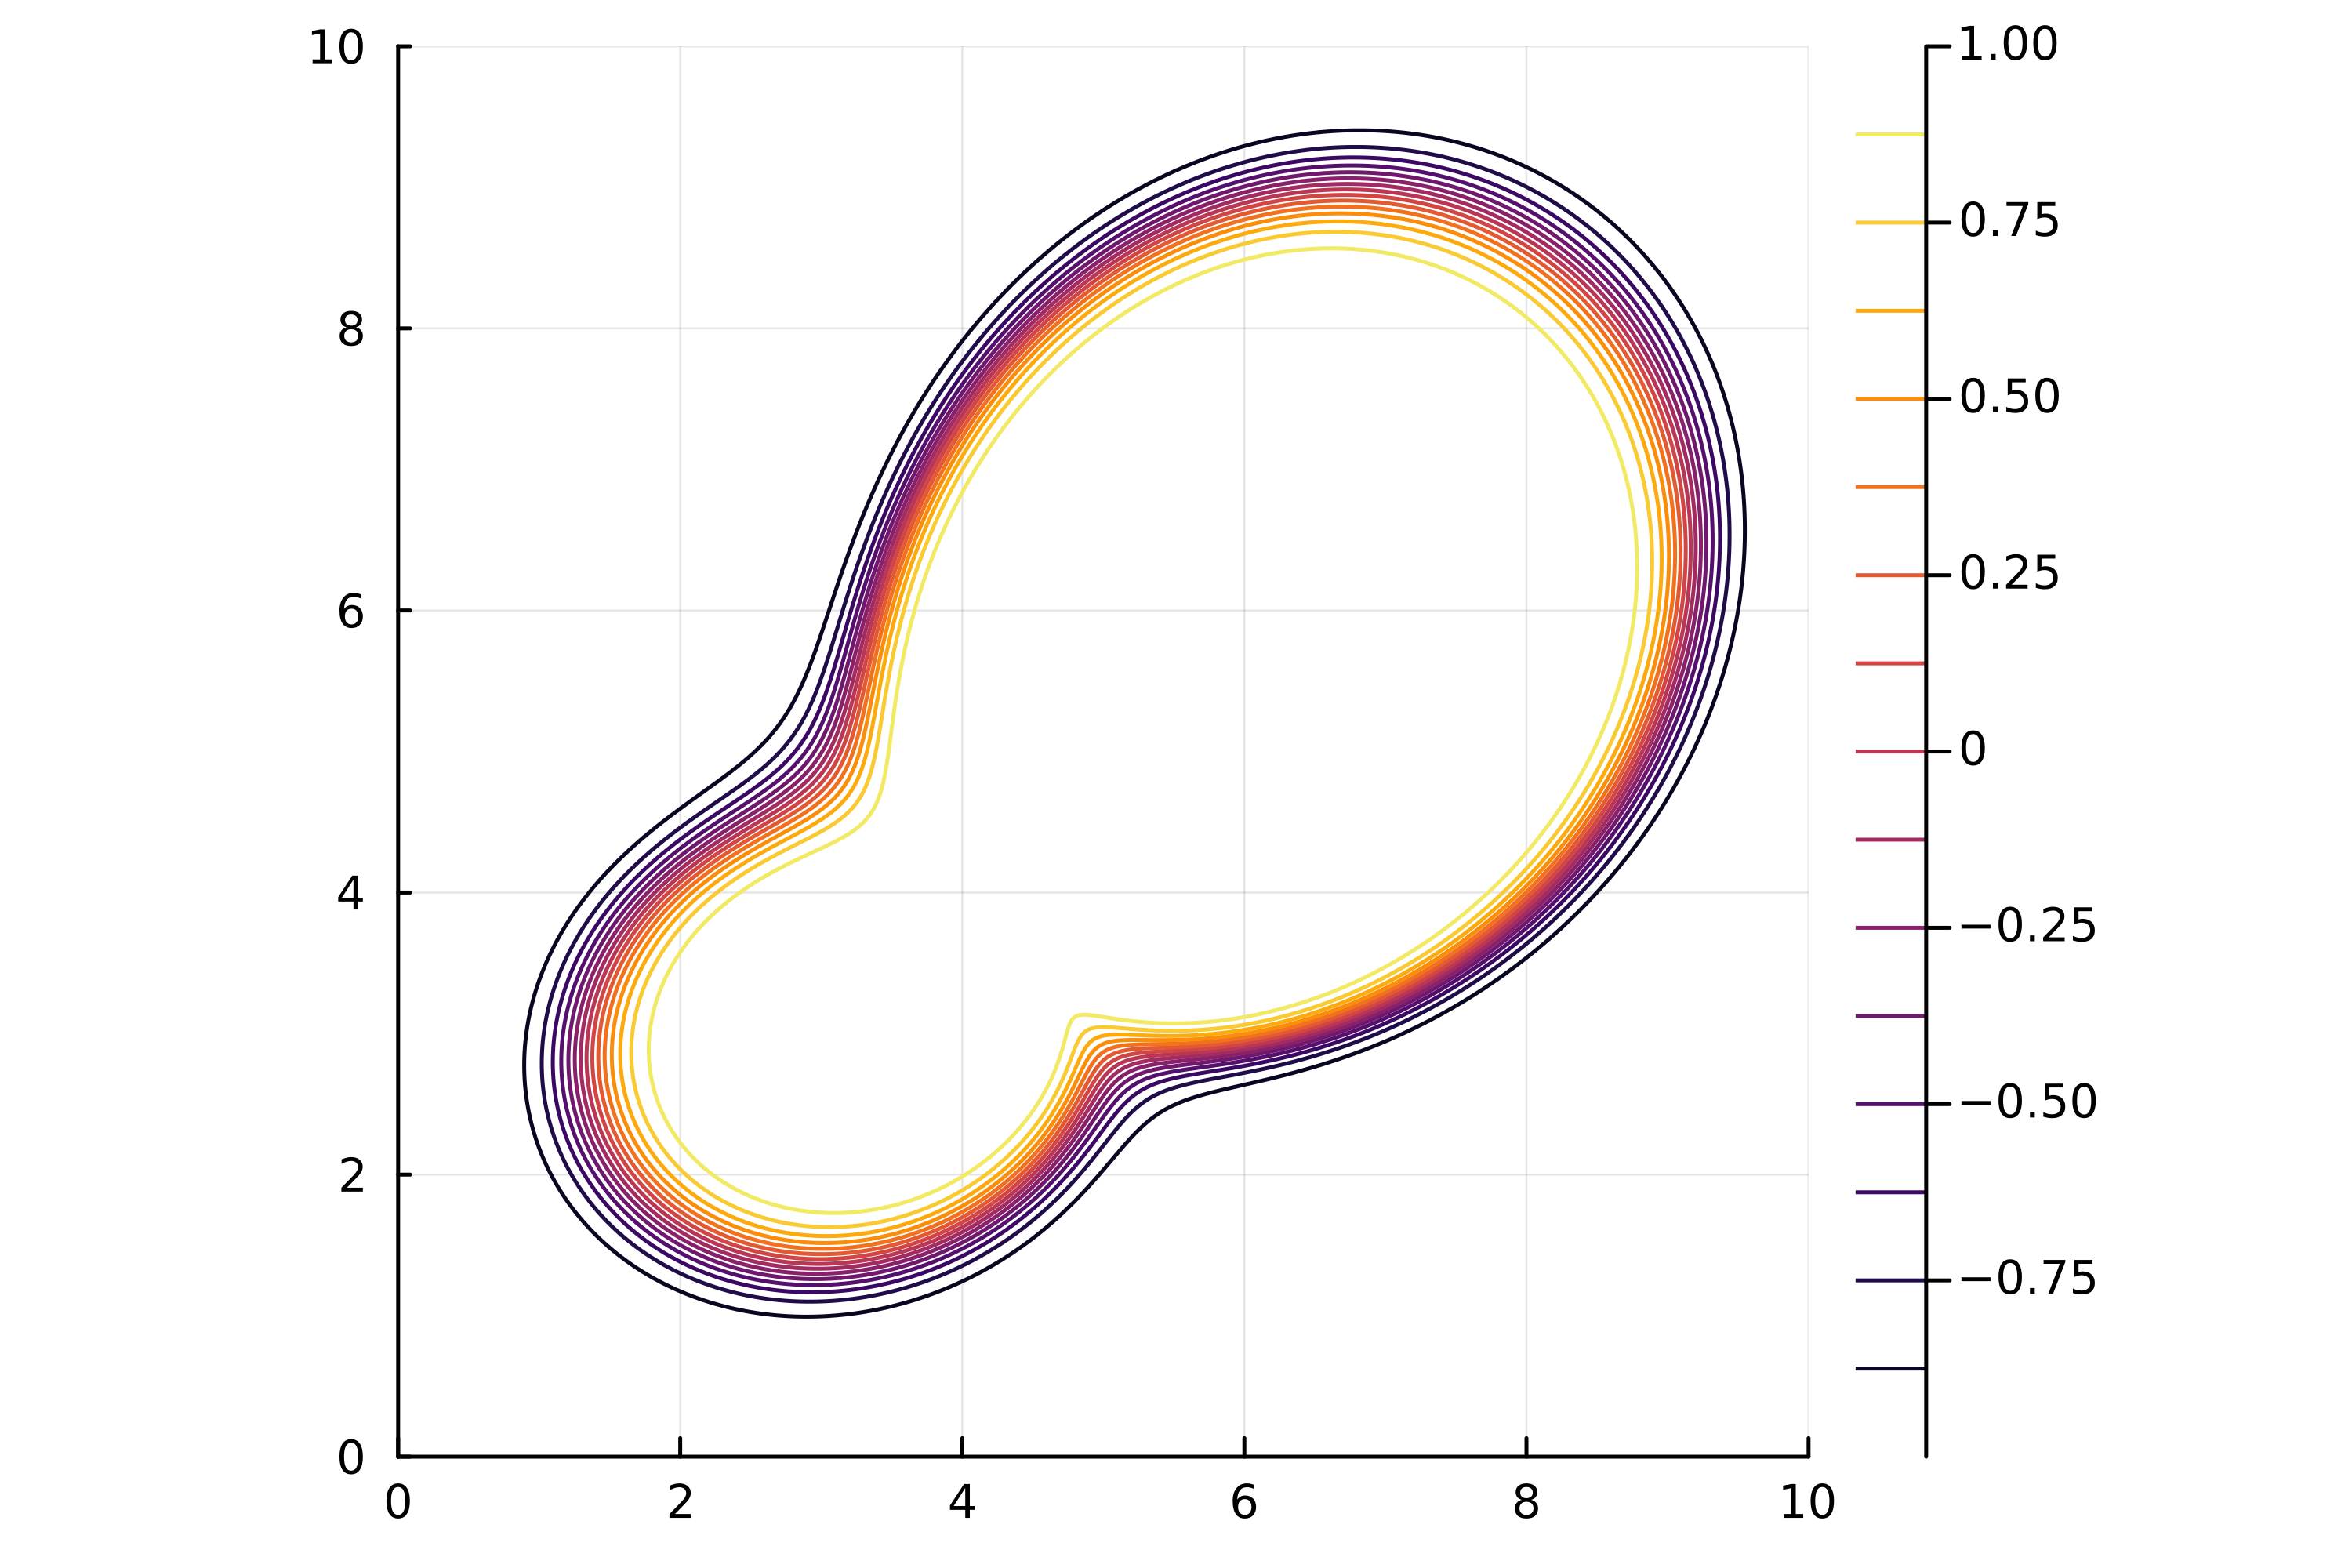
\includegraphics[width=\textwidth]{bachelors-thesis/model_illustrations/PhaseFieldModel.png}
		\caption{A contour plot of a phase field variable $\phi$ illustrates how cells can be modeled through phase field models. The cell's inside is the area where $\phi > 0$. The cell wall sits on the red line where $\phi = 0$. The outer lines display the smooth transition to the outside. }
	\end{subfigure}\hfill
	\begin{subfigure}{0.4\textwidth}
		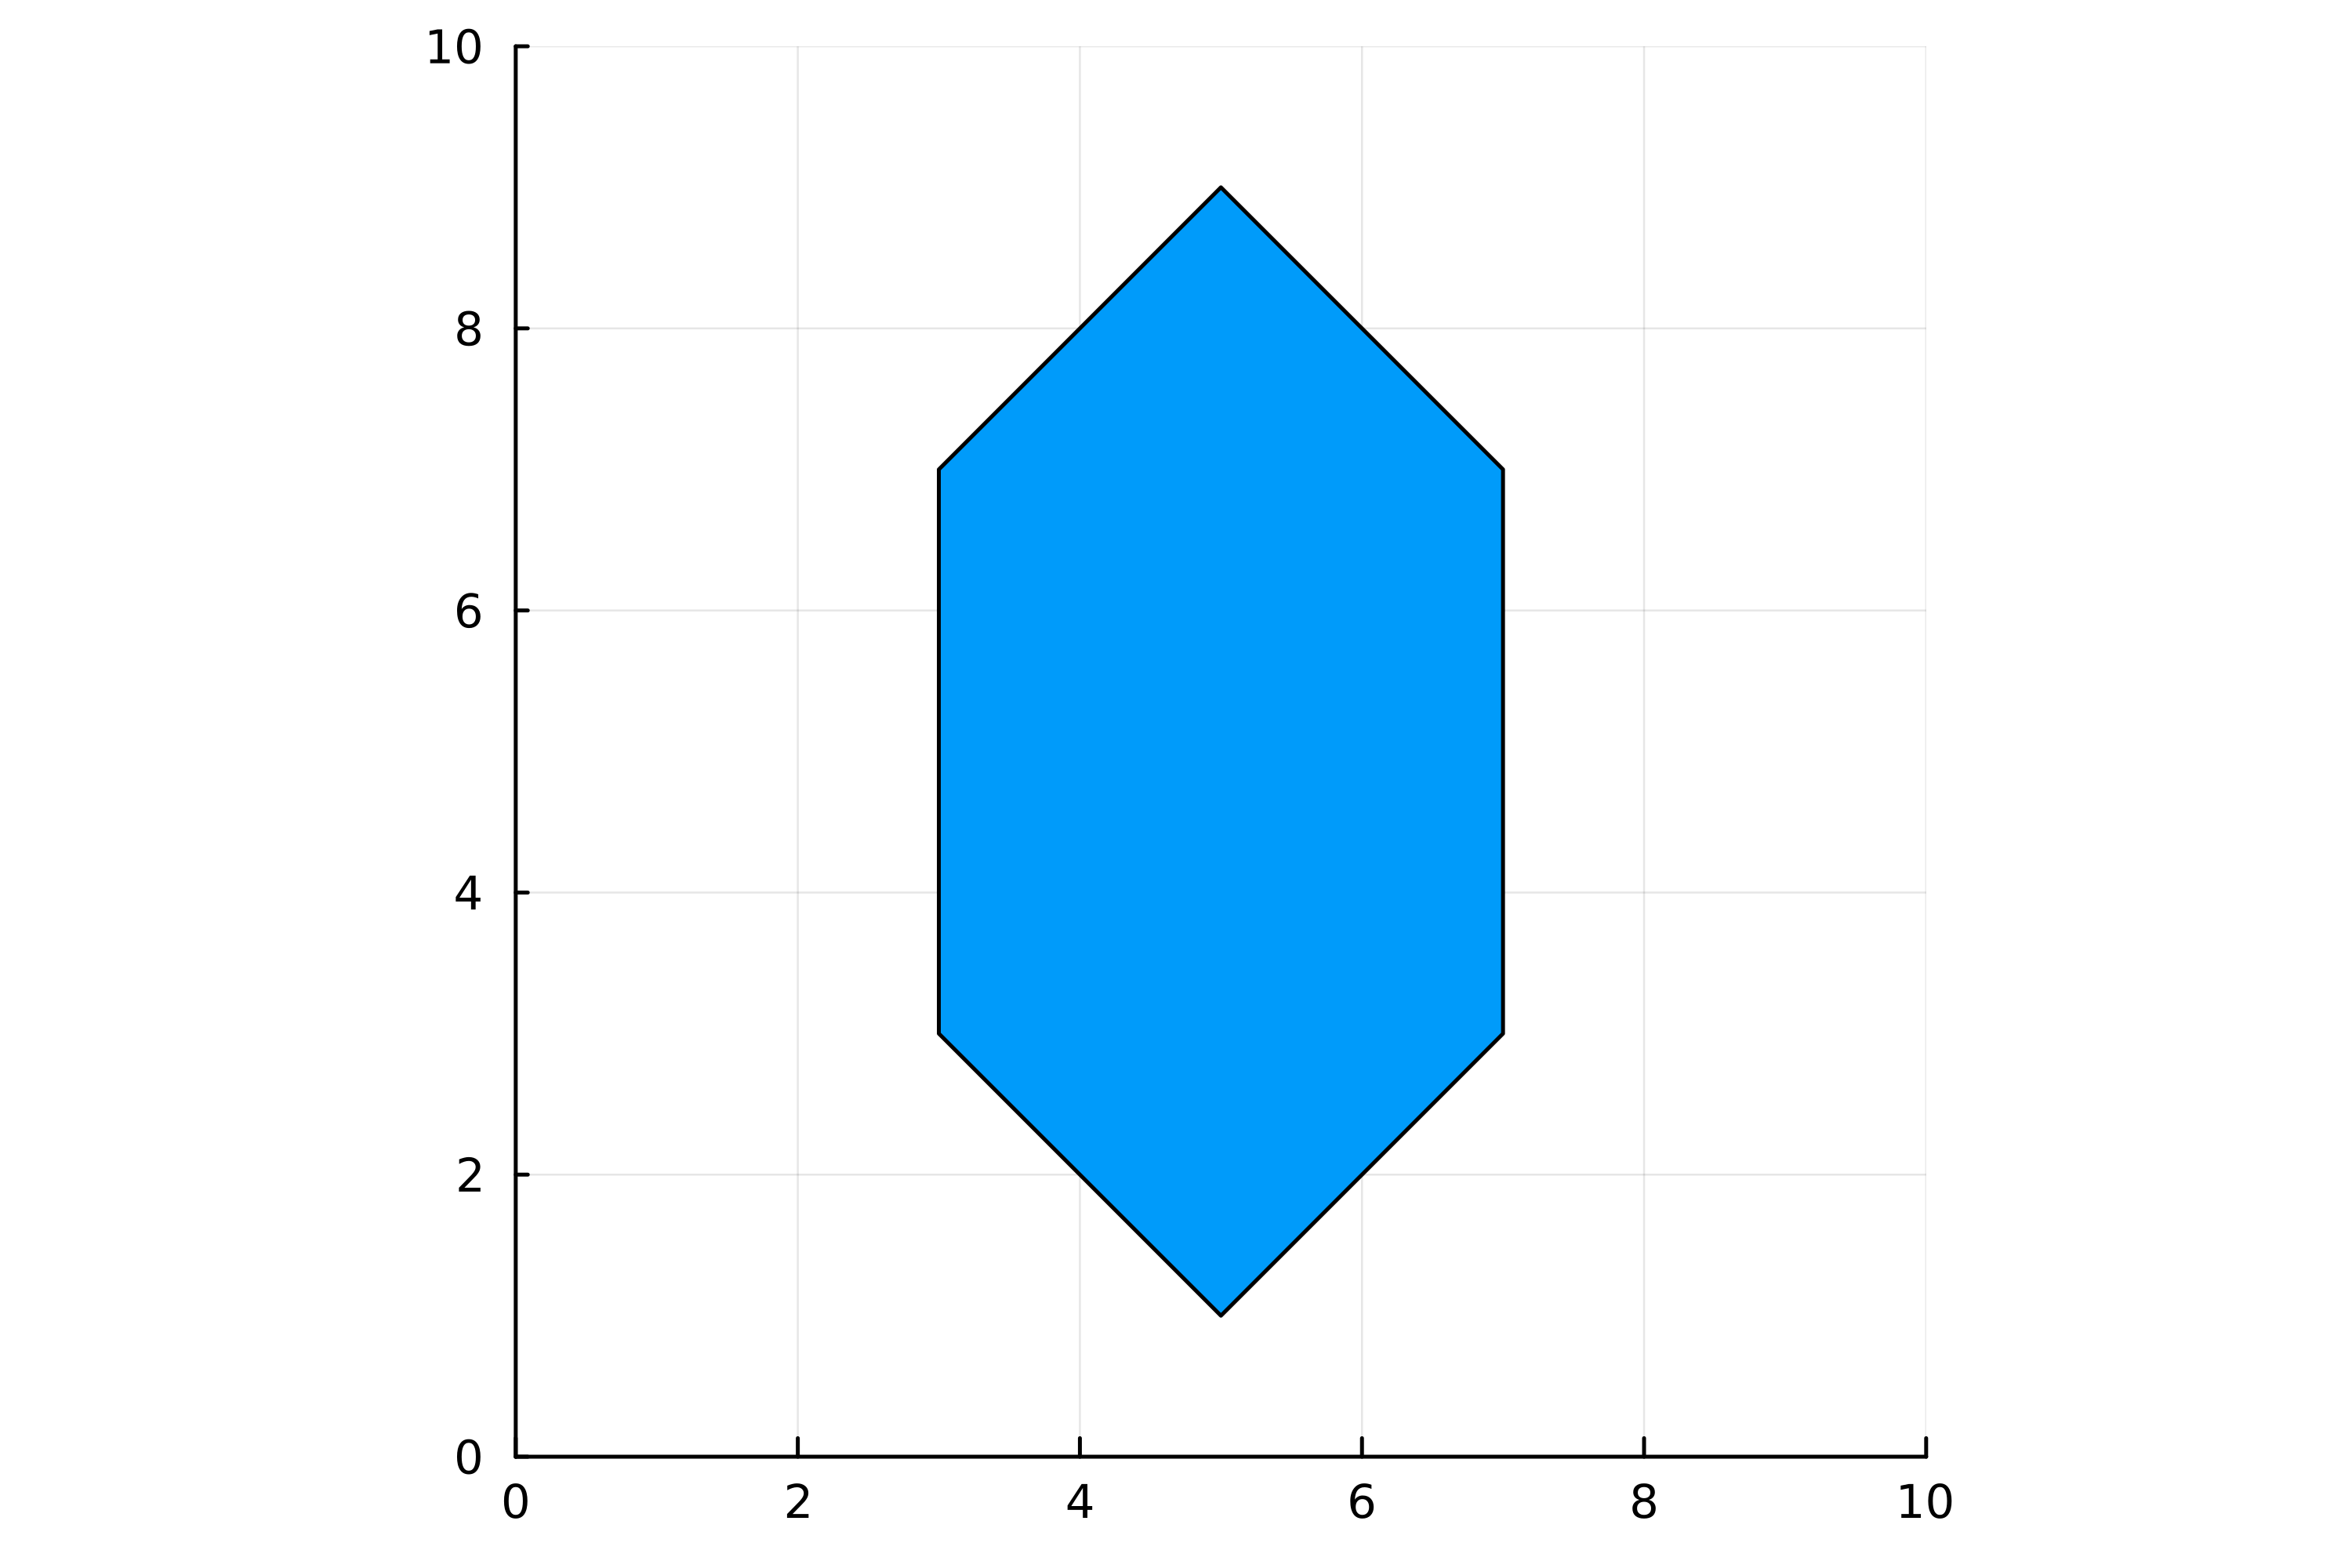
\includegraphics[width=\textwidth]{bachelors-thesis/model_illustrations/VertexModel.png}
		\caption{Another possibility to model cell forms are Vertex models. An example of this is shown here. This cell has six vertices. In order to model cell deformations, one can define forces that act on each vertex separately and thus cause them to move in an according direction. }
	\end{subfigure}
	\caption{To illustrate the models from the introduction, we can see a corresponding plot for each model. The sub figures (a) and (b) are concerned with the representation of cell shapes. In all sub figures, the axes denote the spatial $x$ and $y$ coordinates. } 
	\label{fig:model_illus}
\end{figure}

\newpage 
\subsection*{Derivation of forces}
First, we derived methods for area computation of both models. I will just focus on DF cells from now on. 
For DF cells, we can just apply the \textbf{shoelace lemma}: 
\begin{center}
    $A_C = \sum\limits_{i = 1}^{N} T_i = \frac{1}{2} \sum\limits_{i = 1}^{N} (y_i + y_{i+1})(x_i - x_{i+1}) = \frac{1}{2}\sum\limits_{i = 1}^{N} (x_i y_{i+1} - x_{i+1} y_i) $.
\end{center} 
\begin{figure}[h!]
	% TODO: redo it by myself
    \begin{center}
        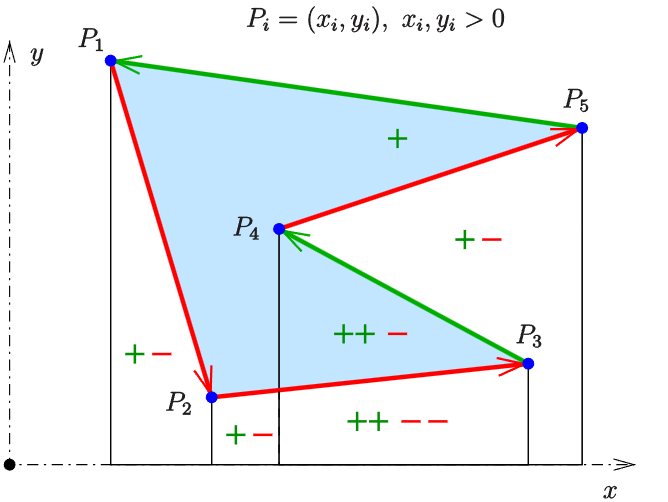
\includegraphics[width=8cm]{bachelors-thesis/shoelace.png}
        \caption{
            This figure shows a geometrical interpretation of the shoelace formula. In difference to the proposition, here the vertices are called $P_i$ and not $\vec{x}_i$. \\
            Source: \cite{ShoelaceFigure2022}}
        \label{fig:shoelace}
    \end{center}
\end{figure}

\newpage
Next, we derived a way to compute the \textbf{overlap} for DF cells: 
\begin{algorithm} \textbf{Computation of a discrete overlaps} \label{alge:discreteOverlap}
	\begin{itemize} 
		\itemsep0em 
		\item[] \text{INPUT:}
		\item Discrete cells  $C$and $\zeta$
		\item List $I$ of unused intersections of $C$ and $\zeta$ 
	\end{itemize}
	\begin{algorithmic}
		\Function{constructOverlap}{$C$, $\zeta$, $I$}		
			\State usedIntersections = List$\{$Intersection$\}$(I[1])
			\State newOverlap = List$\{$Vertices$\}$(I[1])
			\State currentIntersection = I[1]
			
			\For{counter = 1 : length(I)}
			
				\If{counter is even}
					\State newPath, newIntersection = findPath(currentIntersection, $C$, $I$)
				\Else
					\State newPath, newIntersection = findPath(currentIntersection, $\zeta$, $I$)
				\EndIf
				
				\State append!(newOverlap, newPath)
				\If{newIntersection == I[1]} 
					\State \Return newOverlap, usedIntersections
				\Else
					\State append!(newOverlap, newIntersection)
					\State append!(usedIntersections, newIntersection) 
					\State currentIntersection = newIntersection
				\EndIf
			\EndFor
		\EndFunction
	\end{algorithmic}
	\begin{itemize} 
		\itemsep0em 
		\item[] \text{OUTPUT:}
		\item A single intersection `newOverlap' which occurs between $C$ and $\zeta$ and which uses vertices from  $C$ and $\zeta$ as well as only intersections from $I$
		\item A list `usedIntersections' of all intersection that are used in `newOverlap'
	\end{itemize}	
\end{algorithm}

\begin{figure}[h!]
	\centering
	\begin{subfigure}{0.3\textwidth}
		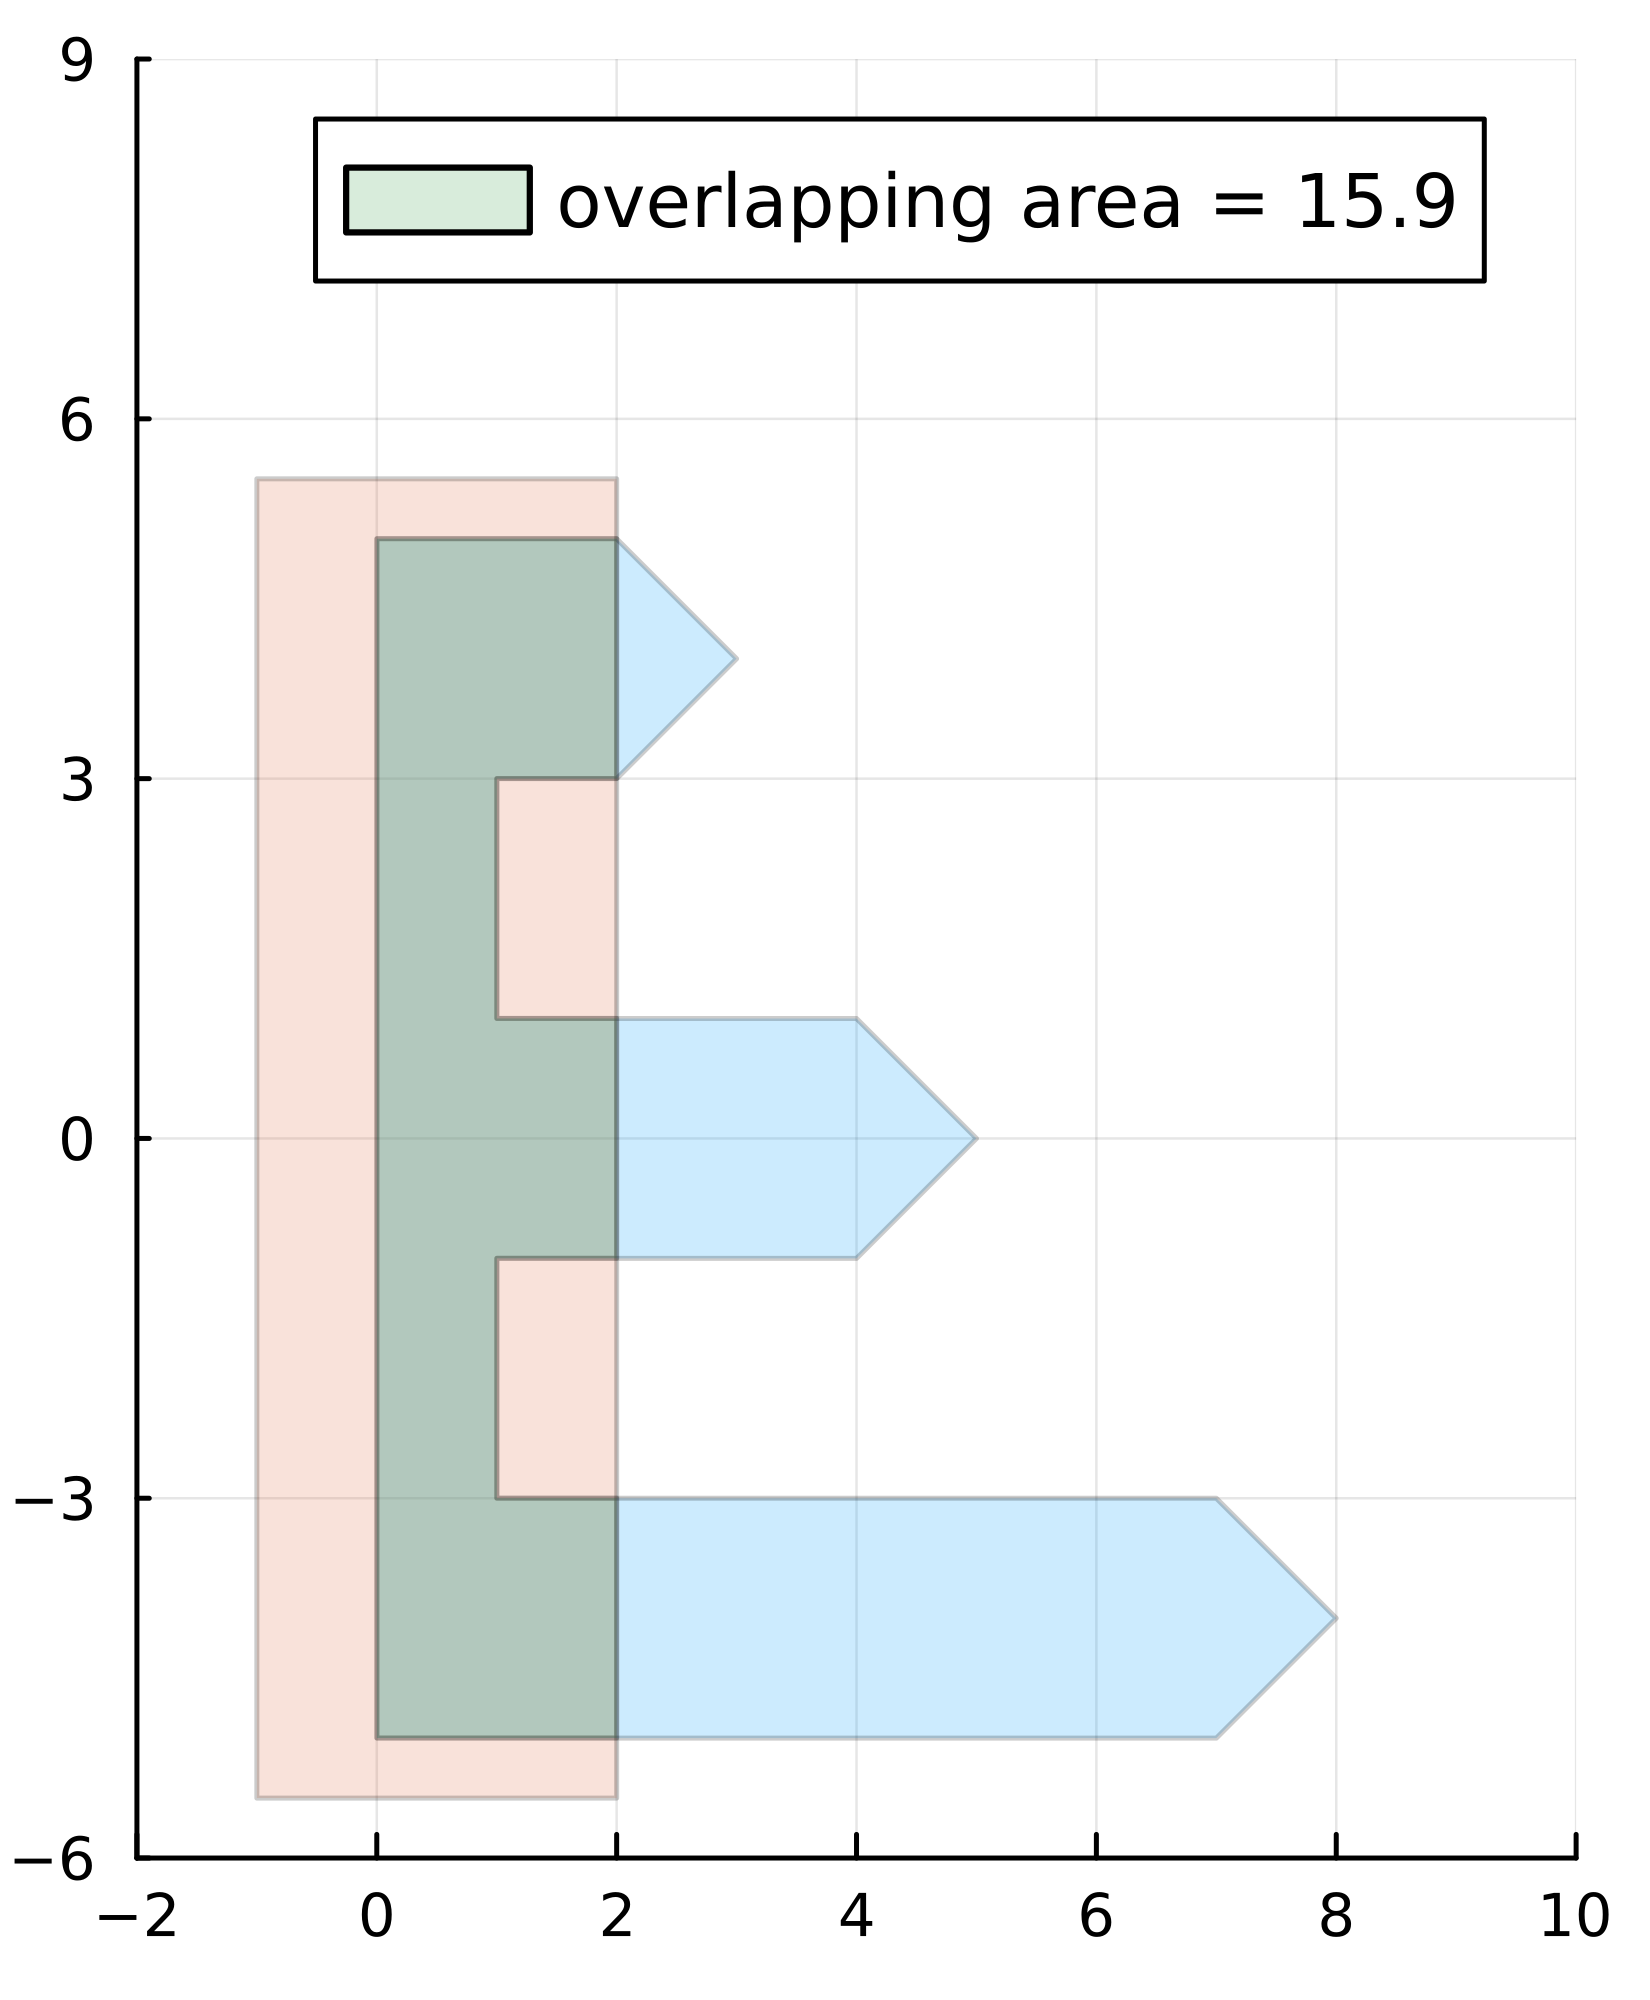
\includegraphics[width=\textwidth]{bachelors-thesis/discreteOverlap/discreteOverlapEx1.png}
	\end{subfigure}
	\hfill
	\begin{subfigure}{0.3\textwidth}
		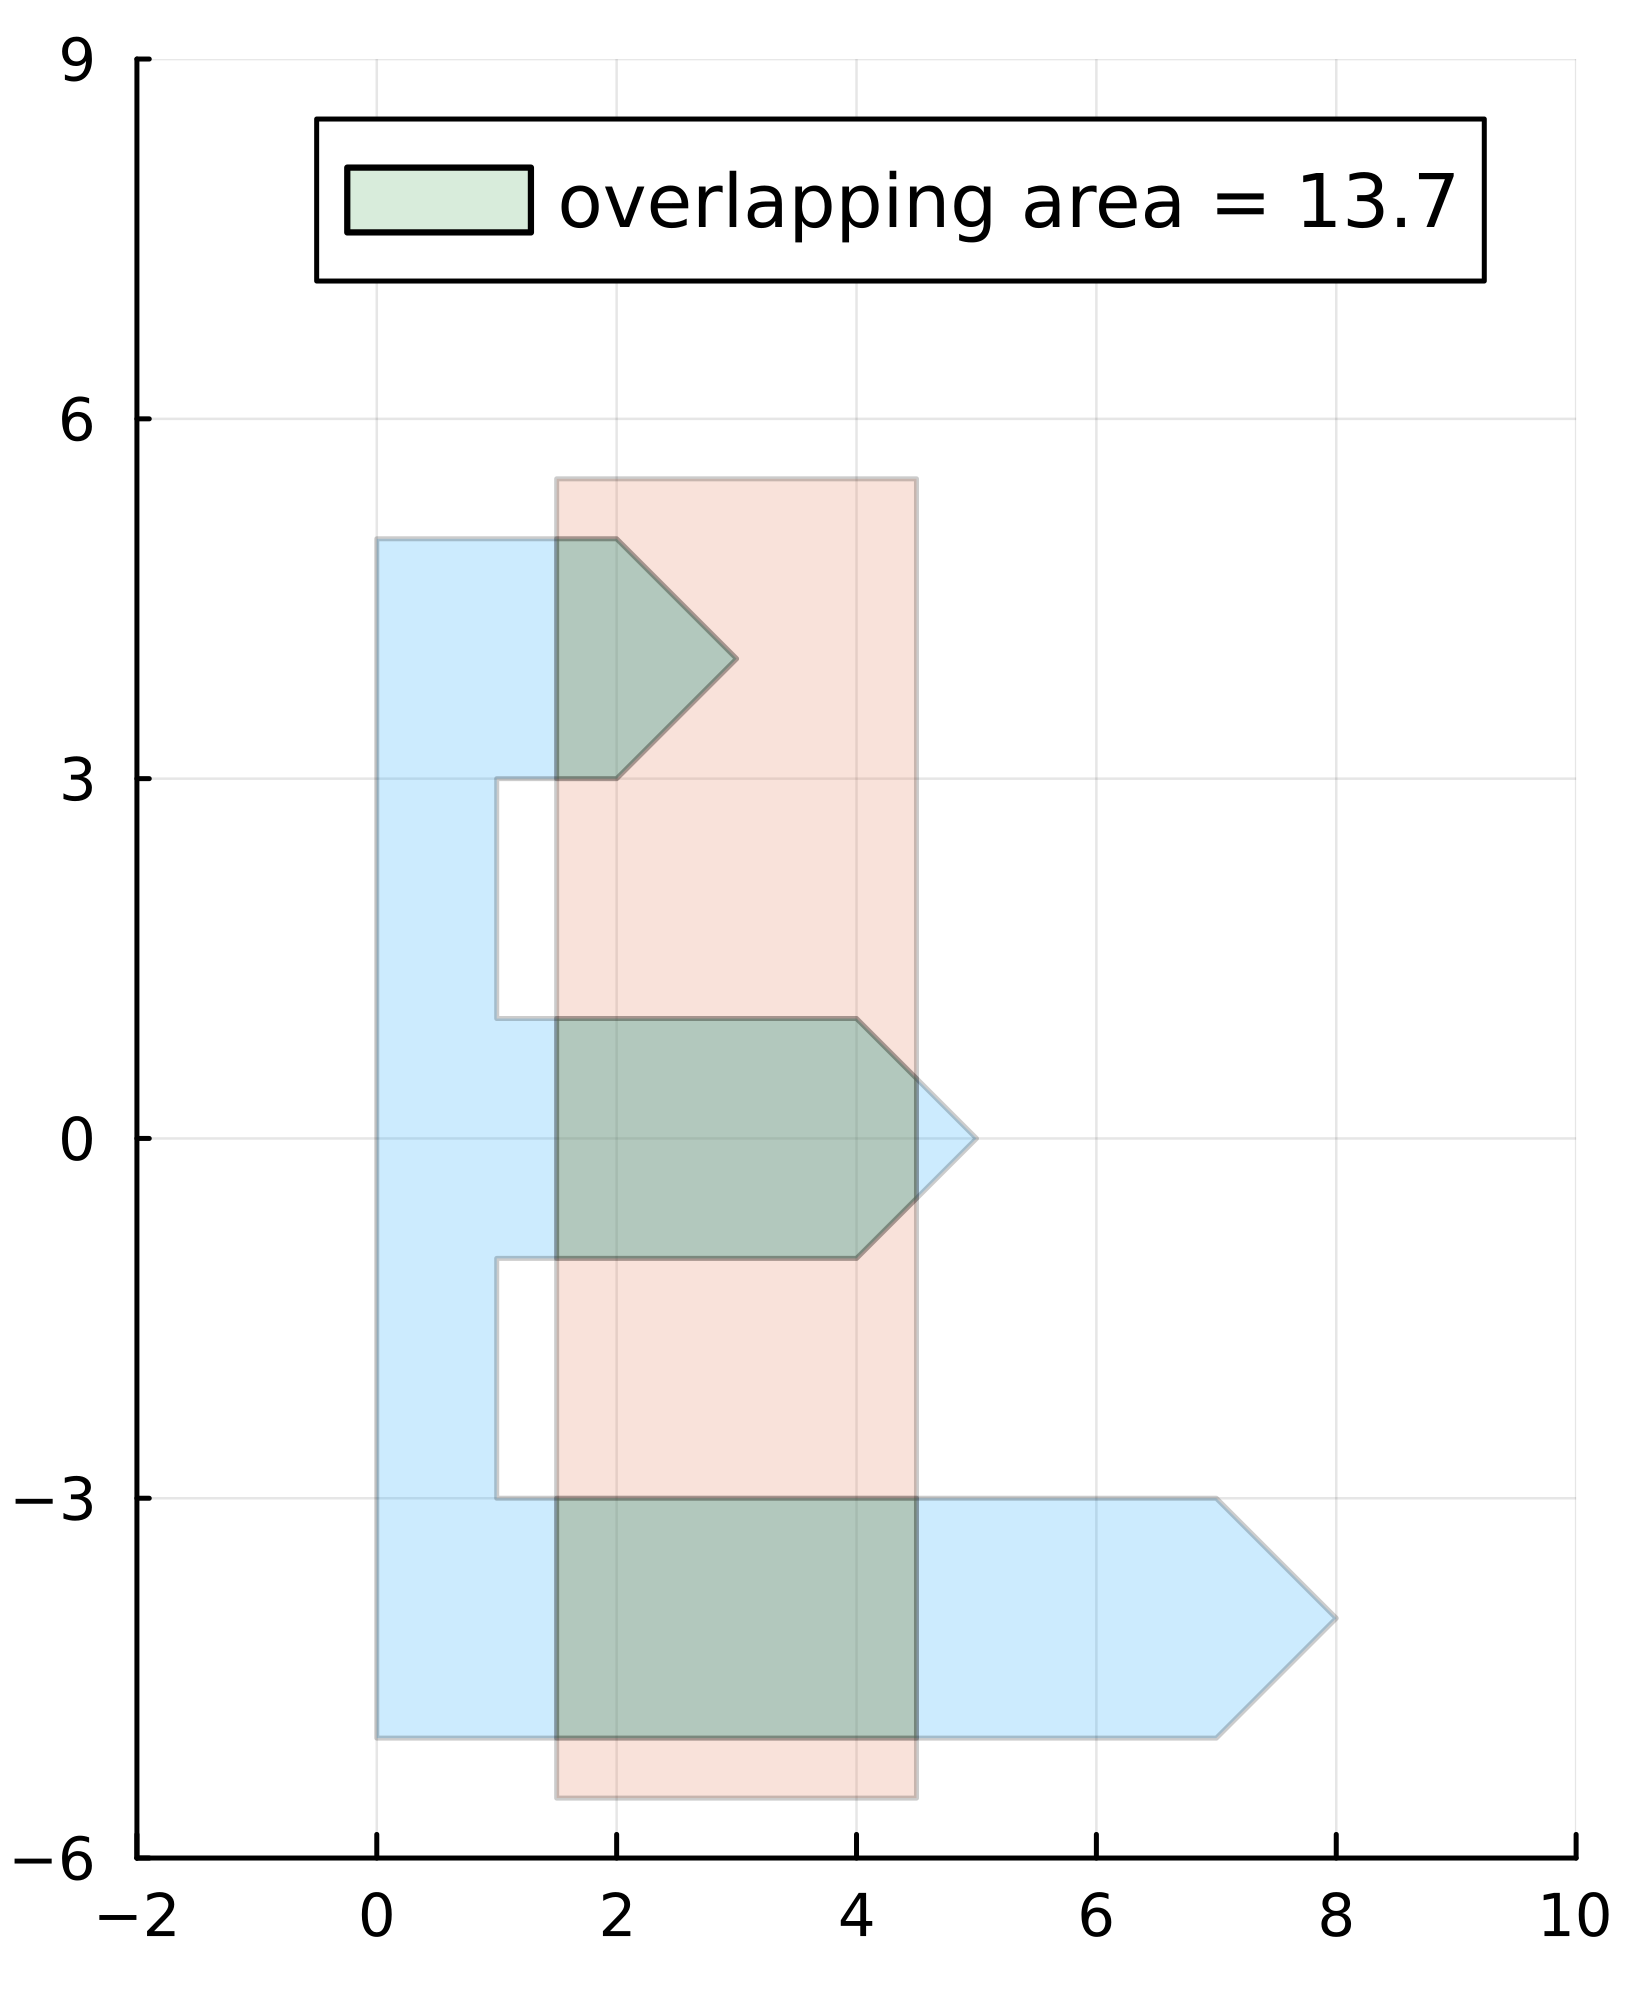
\includegraphics[width=\textwidth]{bachelors-thesis/discreteOverlap/discreteOverlapEx2.png}
	\end{subfigure}
	\hfill
	\begin{subfigure}{0.3\textwidth}
		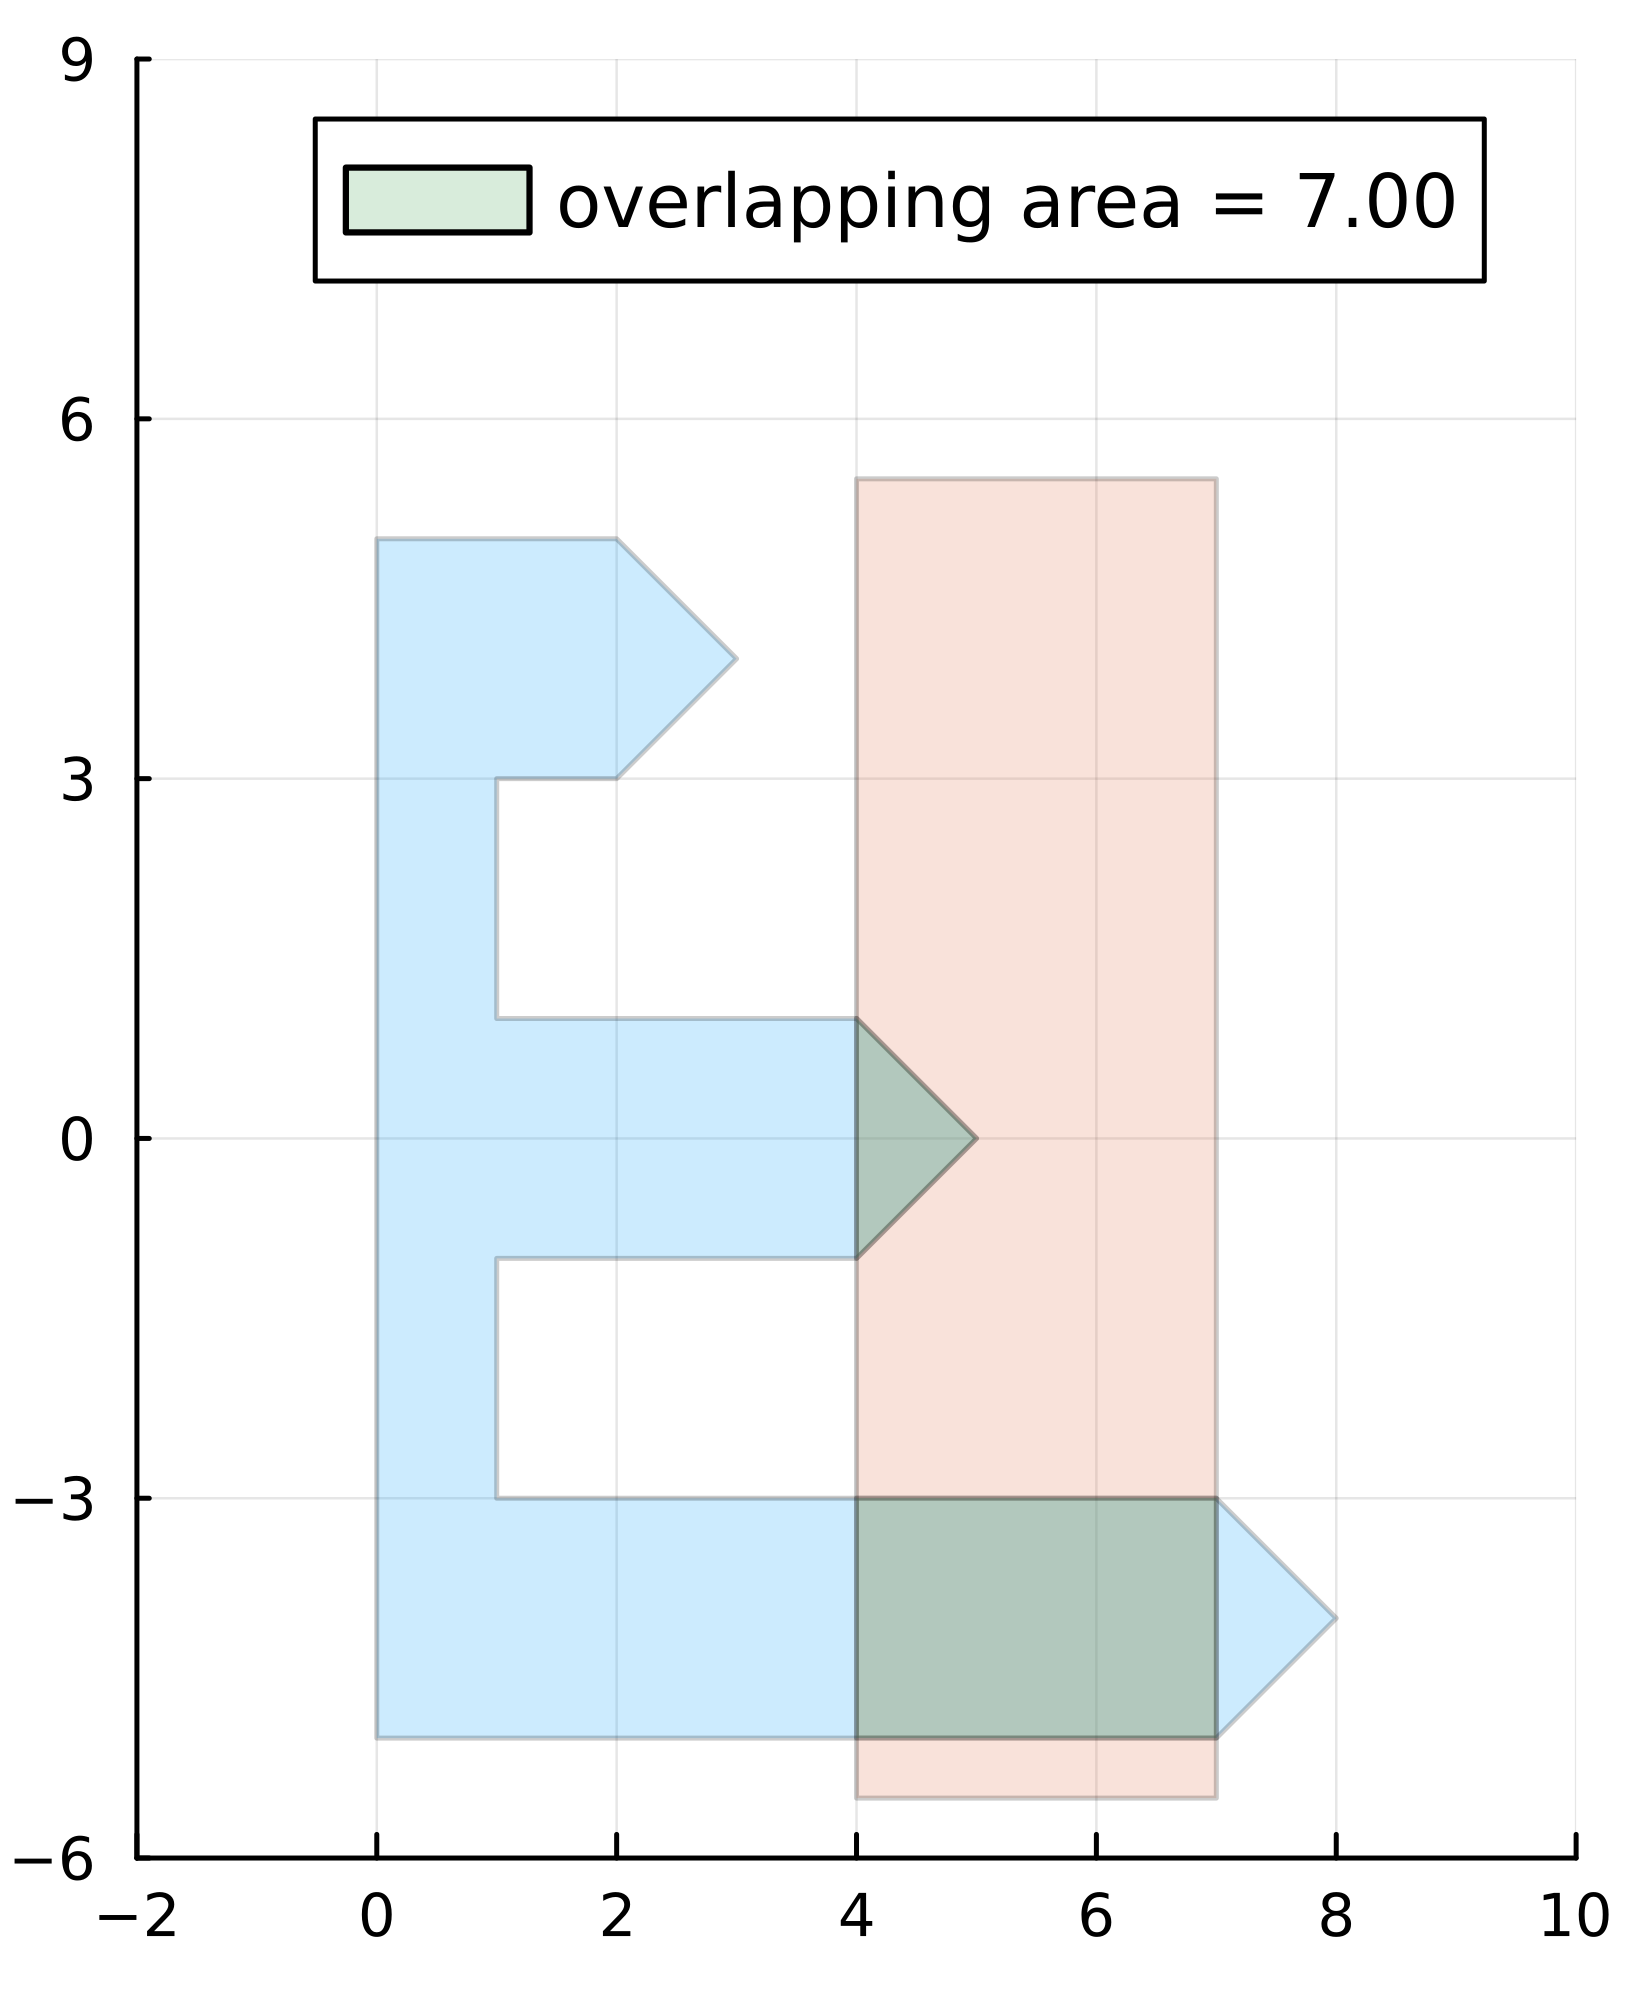
\includegraphics[width=\textwidth]{bachelors-thesis/discreteOverlap/discreteOverlapEx3.png}
	\end{subfigure}\hfill
	\caption{This figure shows 3 plots of 2 DF cells, shown in blue and red, each. One can see the calculated overlap in a green colour and the calculated area of the overlap is shown at the top of the plots. The red cell is shifted to the right in each subsequent plot, resulting in a change of the occurring overlap.}
	\label{fig:finalDiscreteOverlap}
\end{figure}

\newpage 
We defined how our \textbf{forces} look like using energies: 

\begin{definition} \textbf{Force function} \label{def:forceFunction}\\
	For a given energy $E_i$ of the $i$th cell, the force $F_{j}^{(E_i)}$ that describes the impact of $E_i$ on the $j$th vertex of the $i$th cell is given by
	\begin{center}
		$F_{j}^{(E_i)}(\vec{C}) := -\alpha_{E_i}(\vec{C}) \nabla_{\vec{x}_{ij}} E_i(\vec{C})$,
	\end{center}
	where $\alpha_{E_i} > 0$ denotes a positive scaling factor and $\nabla_{\vec{x}_{ij}}$ is the gradient for the $j$th vertex of cell $i$. 	\\
\end{definition}

and introduced the \textbf{area force} ...

\begin{proposition} \textbf{Area force} \\
	The gradient of $A_i$ with respect to the $j$th vertex of cell $i$ is given by 
	\begin{center}
		$\nabla_{\vec{x}_j} A_i(C_i) = \sgn(a(C_i) - a_i^{(d)}) \dfrac{1}{2} \begin{pmatrix} y_{i,j+1} - y_{i,j-1} \\ x_{i,j-1} - x_{i,j+1} \end{pmatrix}$. 
	\end{center}
	As a scaling factor, we choose
	\begin{center}
		$\alpha_{A_i}(C_i) := | a_i^{(d)} - a(C_i) |$. 
	\end{center}
	Thus, the area force reads 
	\begin{align}
		F_{j}^{(A_i)}(C_i) = \frac{1}{2}( a_i^{(d)} - a(C_i)) \begin{pmatrix} y_{i,j+1} - y_{i,j-1} \\ x_{i,j-1} - x_{i,j+1} \end{pmatrix}.
	\end{align}
	Proof.\\
	To reduce the notation effort, we neglect the subscript $i$, because we just consider a single cell.
	In order to compute $\nabla_{\vec{x}_j} | a^{(d)} - a(C) |$, let us first assume that $a^{(d)} \geq a(C)$. Then, one can calculate
	\begin{center}
		$
		\nabla_{\vec{x}_j} | a^{(d)} - a(C) | = - \nabla_{\vec{x}_j} a(C)
		= - \frac{1}{2}\sum\limits_{j = 1}^{N} \nabla_{\vec{x}_j} (x_{j} y_{j+1} - x_{j+1} y_{j})$ \\ \smallskip 
		$=- \frac{1}{2}\sum\limits_{j = 1}^{N} \begin{pmatrix} \partial_{x_j}  (x_{j} y_{j+1} - x_{j+1} y_{j})\\ \partial_{y_j} (x_{j} y_{j+1} - x_{j+1} y_{j})\end{pmatrix} 
		= - \dfrac{1}{2} \begin{pmatrix} y_{j+1} - y_{j-1} \\ x_{j-1} - x_{j+1} \end{pmatrix}
		$
	\end{center}
	
	Remember that $a^{(d)}$ is just an independent constant. In the other case, where $a^{(d)} < a(C(t))$, there is just a change in the sign. The combination of both cases yields the expression above. \\ 
	Since $- | a^{(d)} - a(C) | \sgn(a(C) - a^{(d)}) = a^{(d)} - a(C)$, we can conclude the area force. \\
	\qed
\end{proposition}

... the \textbf{edge force} \dots
\begin{proposition} \textbf{Edge force} \\
	The edge force is given by the formula
	\begin{align}
		F^{(E_{ij})}_j(C_i) = \dfrac{e_{j-1} - e_{i, j-1}^{(d)}}{e_{j-1}(C_i) } \begin{pmatrix} x_{j-1} - x_j \\ y_{j-1} - y_j\end{pmatrix} + 
		\dfrac{e_{j} - e_{i, j}^{(d)}}{e_{j}(C_i)} \begin{pmatrix} x_{j+1} - x_j \\ y_{j+1} - y_j\end{pmatrix}.
	\end{align}
	We choose $\alpha_{E_{ij}} := | e_{ij}^{(d)} - e_j(C_i) |$. \\
	Proof. \\
	Since this force acts on each cell individually, we can neglect the subscript $i$.
	The searched term has the following structure
	\begin{center}
		$F^{(E_{j})}_j(C) = - \alpha_{E_{j-1}} \nabla_{\vec{x}_j} E_{j-1}(C) - \alpha_{E_{j}} \nabla_{\vec{x}_j} E_{j}(C)$,
	\end{center}
	with the scaling factors $\alpha_{E_j}$ already defined in the proposition. \\	
	The partial derivatives of the edge length $e_j$ are
	\begin{center}
		$\partial_{x_j} e_j(C) = \partial_{x_j} ( (x_{j+1}- x_j)^2 + (y_{j+1} - y_j)^2)^{\frac{1}{2}} = \dfrac{ x_j - x_{j+1} }{ e_j(C) }$, \\
		$\partial_{y_j} e_j(C) = \dfrac{ y_j - y_{j+1} }{ e_j(C) }$. \\
	\end{center}
	This yields
	\begin{center}
		$ \nabla_{\vec{x}_j} E_{j} = sgn(e_{j}^{(d)} - e_j(C)) \nabla_{\vec{x}_j} - e_j(C)  = sgn(e_{j}^{(d)} - e_j(C))  \dfrac{1}{  e_j(C) } \begin{pmatrix} x_{j+1} - x_j \\ 	y_{j+1} - y_j \end{pmatrix}$,
	\end{center}
	and analogously
	\begin{center}
		$\nabla_{\vec{x}_j} E_{j-1} = sgn(e_{j-1}^{(d)} - e_{j-1}(C_i))  \dfrac{1}{  e_{j-1}(C) } \begin{pmatrix} x_{j-1} - x_j \\ 	y_{j-1} - y_j \end{pmatrix}$. 
	\end{center}
	This yields the edge force 
	\begin{center}
		$F_j^{(E_{j})}(C) = \dfrac{e_{j-1}(C) - e_{j-1}^{(d)}}{e_{j-1}(C)} 
		\begin{pmatrix}  x_{j-1} - x_j \\ y_{j-1} - y_j  \end{pmatrix} + 
		\dfrac{e_{j}(C) - e_{j}^{(d)}}{e_{j}(C)} 
		\begin{pmatrix}  x_{j+1} - x_j \\ y_{j+1} - y_j  \end{pmatrix}$.
	\end{center}
	\qed  
\end{proposition}

\dots the \textbf(interior angle force) \dots

\begin{proposition} \textbf{Interior angle force} \\
	The interior angle force is given by
	\begin{center}
		$F^{(I_{ij})}_j(C_i) = (\iota_{ij}^{(d)} - \iota_j(C_i))\left(
		\dfrac{1}{\norm[\vec{v}_1]^2} \begin{pmatrix}
			v_{1,y} \\-v_{1,x}
		\end{pmatrix}
		+ \dfrac{1}{\norm[\vec{v}_2]^2}\begin{pmatrix} -v_{2,y} \\ v_{2,x} \end{pmatrix}\right)
		$,
	\end{center}
	where $\vec{v}_1 = (v_{1,x}, v_{1,y})^T :=\vec{x}_{j-1} - \vec{x}_{j}$ and  $\vec{v}_2 = (v_{2,x}, v_{2,y})^T := \vec{x}_{j+1} - \vec{x}_{j}$. \\
	The scaling factor is defined as $\alpha_{I_{ij}} := | \iota_{ij}^{(d)} - \iota_j(C) |$. \\
	Proof. \\
	Again, we neglect the $i$, because we just consider one cell. 
	The goal is to determine the interior angle force
	\begin{center}
		$
		F^{(I_j)}_j(C) = - |\iota_{j}^{(d)} - \iota_j(C)| \nabla_{\vec{x}_j}I_j(C)
		$
	\end{center}
	Just like in the last forces, we use the $\sgn$ function to get rid of the absolute value, yielding
	\begin{center}
		$
		\nabla_{\vec{x}_j} I(C) = \sgn(\iota_j^{(d)}-\iota_j(C)) \nabla_{\vec{x}_j} (- \iota_j(C))
		$,
	\end{center}
	since the desired state is just a constant number. Since we have a minus in front of the gradient at the end of the equation, the searched force can be written as 
	\begin{center}
		$
		F^{(I_j)}_j(C) = (\iota_{j}^{(d)} - \iota_j(C)) \nabla_{\vec{x}_j}\iota_j(C)
		$.
	\end{center}
	The gradient of $\iota_j(C)$ is still missing. We will neglect the not differentiable modulo operator and must then compute
	\begin{center}
		$
		\nabla_{\vec{x}_j} (\atanxy(\vec{v}_1(C)) - \atanxy(\vec{v}_2(C))), 
		$
	\end{center}
	where $\vec{v}_1(C) = (x_{j-1} - x_{j} , y_{j-1} - y_{j})^T$ and $\vec{v}_2(C) = (x_{j+1} - x_{j} , y_{j+1} - y_{j})^T$. \\
	The function $\atanxy$ is partly defined and not truly differentiable. We still want to compute a gradient to use it for our interior angle force. Since $\atanxy(x,y) = \arctan(\frac{y}{x}) + \; constant$ almost everywhere, we will use the function $g(x,y) = \arctan(\frac{y}{x})$ for the derivation, because the different constants do not matter in the derivation. With $g$, we can rewrite $\iota_j(C) =g(x,y) \circ \vec{v}_1(C) - g(x,y) \circ \vec{v}_2(C) $. \\
	Thus, we need to determine 
	\begin{center}
		$
		\nabla_{\vec{x}_j} (g(x,y) \circ \vec{v}_1(C) - g(x,y) \circ \vec{v}_2(C)).
		$
	\end{center}
	The partial derivatives of $g$ are
	\begin{center}
		$\partial_{x} \arctan(\frac{y}{x}) = - \dfrac{y}{x^2} \dfrac{1}{1 + (\frac{y}{x})^2} = - \dfrac{y}{x^2 + y^2}$, \\
		$\partial_{y} \arctan(\frac{y}{x}) =  \dfrac{1}{x} \dfrac{1}{1 + (\frac{y}{x})^2} =  \dfrac{x}{x^2 + y^2}$.
	\end{center}
	It is easy to see that 
	\begin{center}
		$
		\partial_{x_j} \vec{v}_1(C) = \partial_{x_j} \vec{v}_2(C) = (-1,0)^T,
		\partial_{y_j} \vec{v}_1(C) = \partial_{y_j} \vec{v}_2(C) = (0, -1)^T. 
		$
	\end{center}
	This implies
	\begin{figure}[b!]
		\begin{center}
			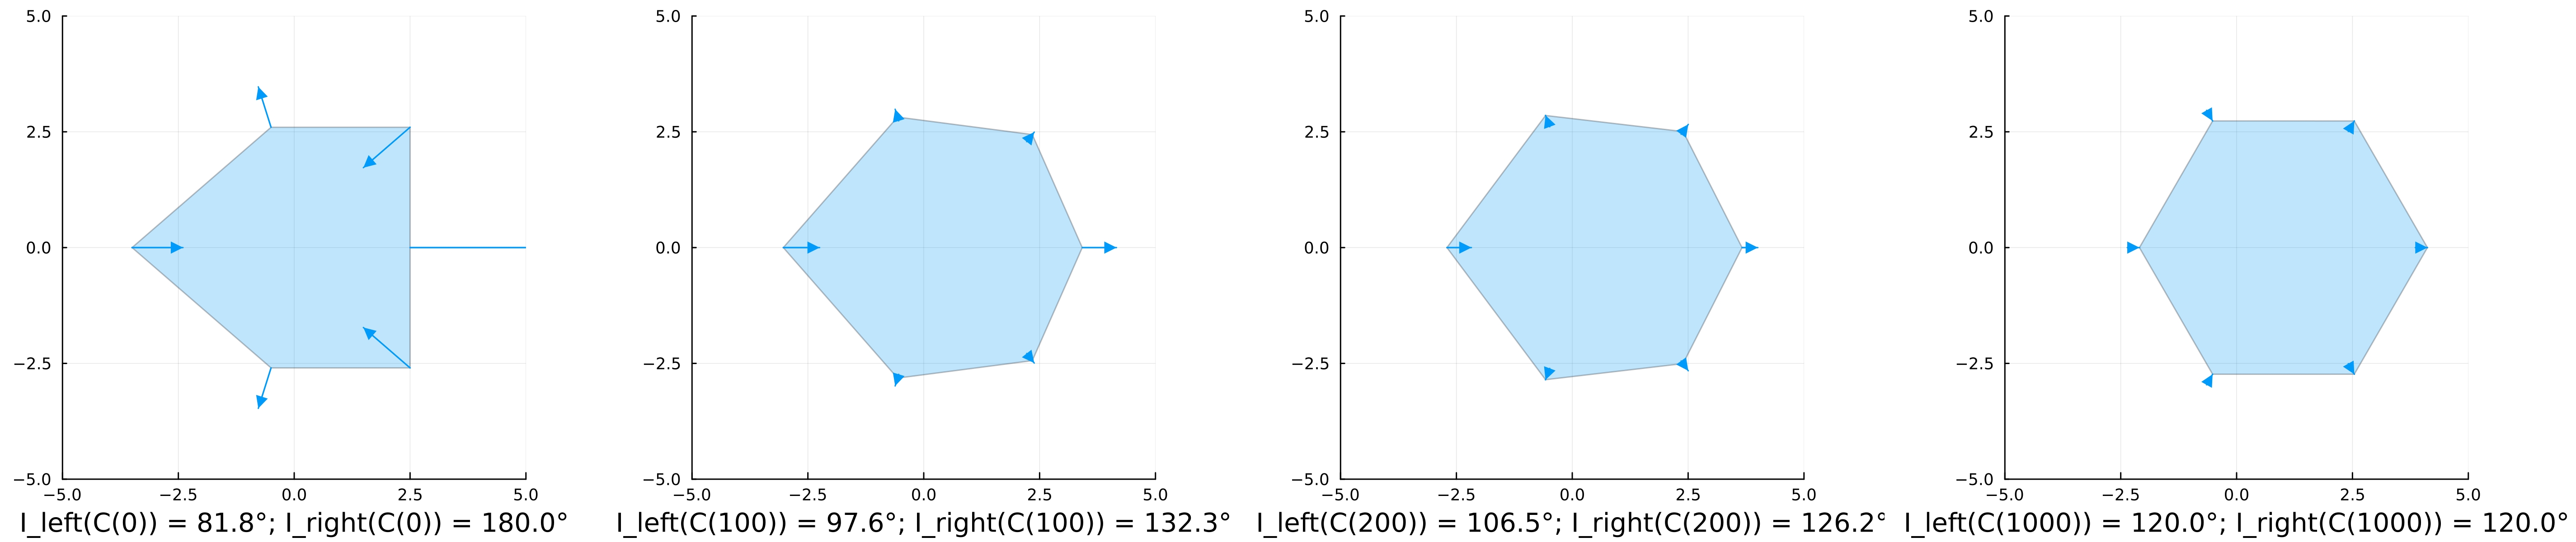
\includegraphics[width=15cm]{bachelors-thesis/forces/angle/angle1.png}
			\caption{This figure shows how the interior angle force acts on the vertices of a DF cell. The initial state can be seen in the first diagram. The desired state is the horizontally mirrored version of the initial state. Below each chart, we can see the current interior angles at $t \in \{0,50,100,3000\}$ of the two vertices that have the $y$ value zero. The desired states are $90$° for the right and $270$° for the left considered vertex. The interior angle force ensures that each interior angle transitions to the desired state over time, as we can see in this figure. }
			\label{fig:angleForce}
		\end{center}
	\end{figure}
	\begin{center}
		$
		\partial_{x_j} \iota_j(C) 
		\corresponds \partial_{x_j}( g\circ \vec{v}_1(C) - g \circ \vec{v}_2(C))$ \\ \smallbreak	
		$= (g'(\vec{v}_1(C)) \partial_{x_j} \vec{v}_1(C) - g'(\vec{v}_2(C))\partial_{x_j} \vec{v}_2(C) $ \\ \smallbreak	
		$= -(\partial_x g)(\vec{v}_1(C)) + (\partial_x g)(\vec{v}_2(C))$\\ \smallbreak 
		$= \dfrac{ v_{1,y} }{ v_{1,x}^2 + v_{1,y}^2 } - \dfrac{v_{2,y}}{v_{2,x}^2 + v_{2,y}^2}
		$,
	\end{center}
	using the multidimensional chain rule. In a similar fashion, we obtain
	\begin{center}
		$
		\partial_{y_j} \iota_j(C) = -\dfrac{v_{1,x}}{v_{1,x}^2 + v_{1,y}^2} + \dfrac{v_{2,x}}{v_{2,x}^2 + v_{2,y}^2}.
		$
	\end{center}
	Together this yields
	\begin{center}
		$
		\nabla_{\vec{x}_j} \iota_j(C) = \dfrac{1}{\norm[\vec{v}_1]^2} \begin{pmatrix} v_{1,y} \\ - v_{1,x} \end{pmatrix} + 
		\dfrac{1}{\norm[\vec{v}_2]^2} \begin{pmatrix} -v_{2,y} \\ v_{2,x} \end{pmatrix},
		$
	\end{center}
	which corresponds to the term from the proposition.\\
	\qed 
\end{proposition}

\dots and last but not least the \textbf{overlap force}

\begin{proposition} \textbf{Overlap force} \\
    The overlap force $F_j^{(O_i)}$ that acts on $\vec{x}_{ij}$ is given by
   \begin{align}
       F_j^{(O_i)}(\vec{C}) = \sum\limits_{m=1, m\neq i}^{M} ( \sum\limits_{D_k \in \Omega_{im}} - \mathbbm{1}_{\omega_{ik}}(\vec{x}_{ij})  a(D_k)\nabla_{\vec{d}_{l}} a(D_k)),
   \end{align}
   with $\nabla_{\vec{d}_{l}} a(D_k)$ given as
   \begin{center}
       $\nabla_{\vec{d}_{l}} a(D_k) = 
           \dfrac{1}{2}\begin{pmatrix}	d_{l+1}^{y} - d_{l-1}^{y} \\d_{l-1}^{x} - d_{l+1}^{x}	\end{pmatrix},
       $
   \end{center}
   with $\vec{d}_{l}$ being the corresponding vertex to $\vec{x}_{ij}$ in the according overlap and $\vec{d}_{l-1}$ and $\vec{d}_{l+1}$ being the vertices before and after $\vec{d}_{l}$. \\
   Proof. \\
   Instead of just using one scaling factor for each vertex, we will use a scaling factor $\alpha_{O_i, D_k} = a(D_k)$ for each individual overlap $D_k$. \\
   For all vertices $\vec{x}_{ij} \notin \omega_{ik}$, that are not included in the overlap $D_k$, the force is zero, because a change of position would not impact the area of the overlap in this case. This produces the indicator function $\mathbbm{1}_{\omega_{ik}}(\vec{x}_{ij})$ in the formula, that makes the force vanish for $\vec{x}_{ij} \notin \omega_{ik}$. \\
   Per definition of $\omega_{ik}$, we can always find an overlap vertex $\vec{d}_l$ that corresponds to $\vec{x}_{ij}$ if $\vec{x}_{ij} \in \omega_{ik}$. In this case, we can apply the gradient with respect to $\vec{d}_l$ on the area functional of $D_k$, to compute the direction of the fastest descent. \\	
   Thus, we must solve 
   \begin{center}
       $
       F_j^{(O_i)}(\vec{C}) = \sum\limits_{l=1, l\neq i}^{M} ( \sum\limits_{D_k \in \Omega_{il}} -\mathbbm{1}_{\omega_{ik}}(\vec{x}_{ij}) a(D_k) \nabla_{\vec{d}_l} a(D_k)).
       $
   \end{center}
   We can use the gradient computation shown in the area force, to determine
   \begin{center}
       $
       \nabla_{\vec{d}_l} a(D_k) = \frac{1}{2} 
       \begin{pmatrix}	d_{l+1}^{y} - d_{l-1}^{y} \\d_{l-1}^{x} - d_{l+1}^{x}	\end{pmatrix}
       $.
   \end{center}
   \qed
\end{proposition}

\newpage 
\subsection*{The interactive system} 
\begin{model} \textbf{First interacting system} \label{model:interaction1}\\ 
	The sum of all derived forces yields the first interacting system
	\begin{align}
		d\vec{x}_{ij}(t) =  F^{(A_i)}_j(C_i) + F^{(E_{ij})}_j(C_i) +F^{(I_{ij})}_j(C_i) +10 F^{(O_i)}_j(C_i) + \sqrt{2D} dB_t^{(i)}, \label{eq:interaction1}
	\end{align}
	where $\vec{x}_{ij}$ again stands for the vertex $j$ of the $i$th cell, $(1\leq i \leq9, \; 1\leq j \leq 20)$. 
\end{model}

and then made a rescaling which balanced all forces 
\begin{figure}[h!]
	\begin{center}
		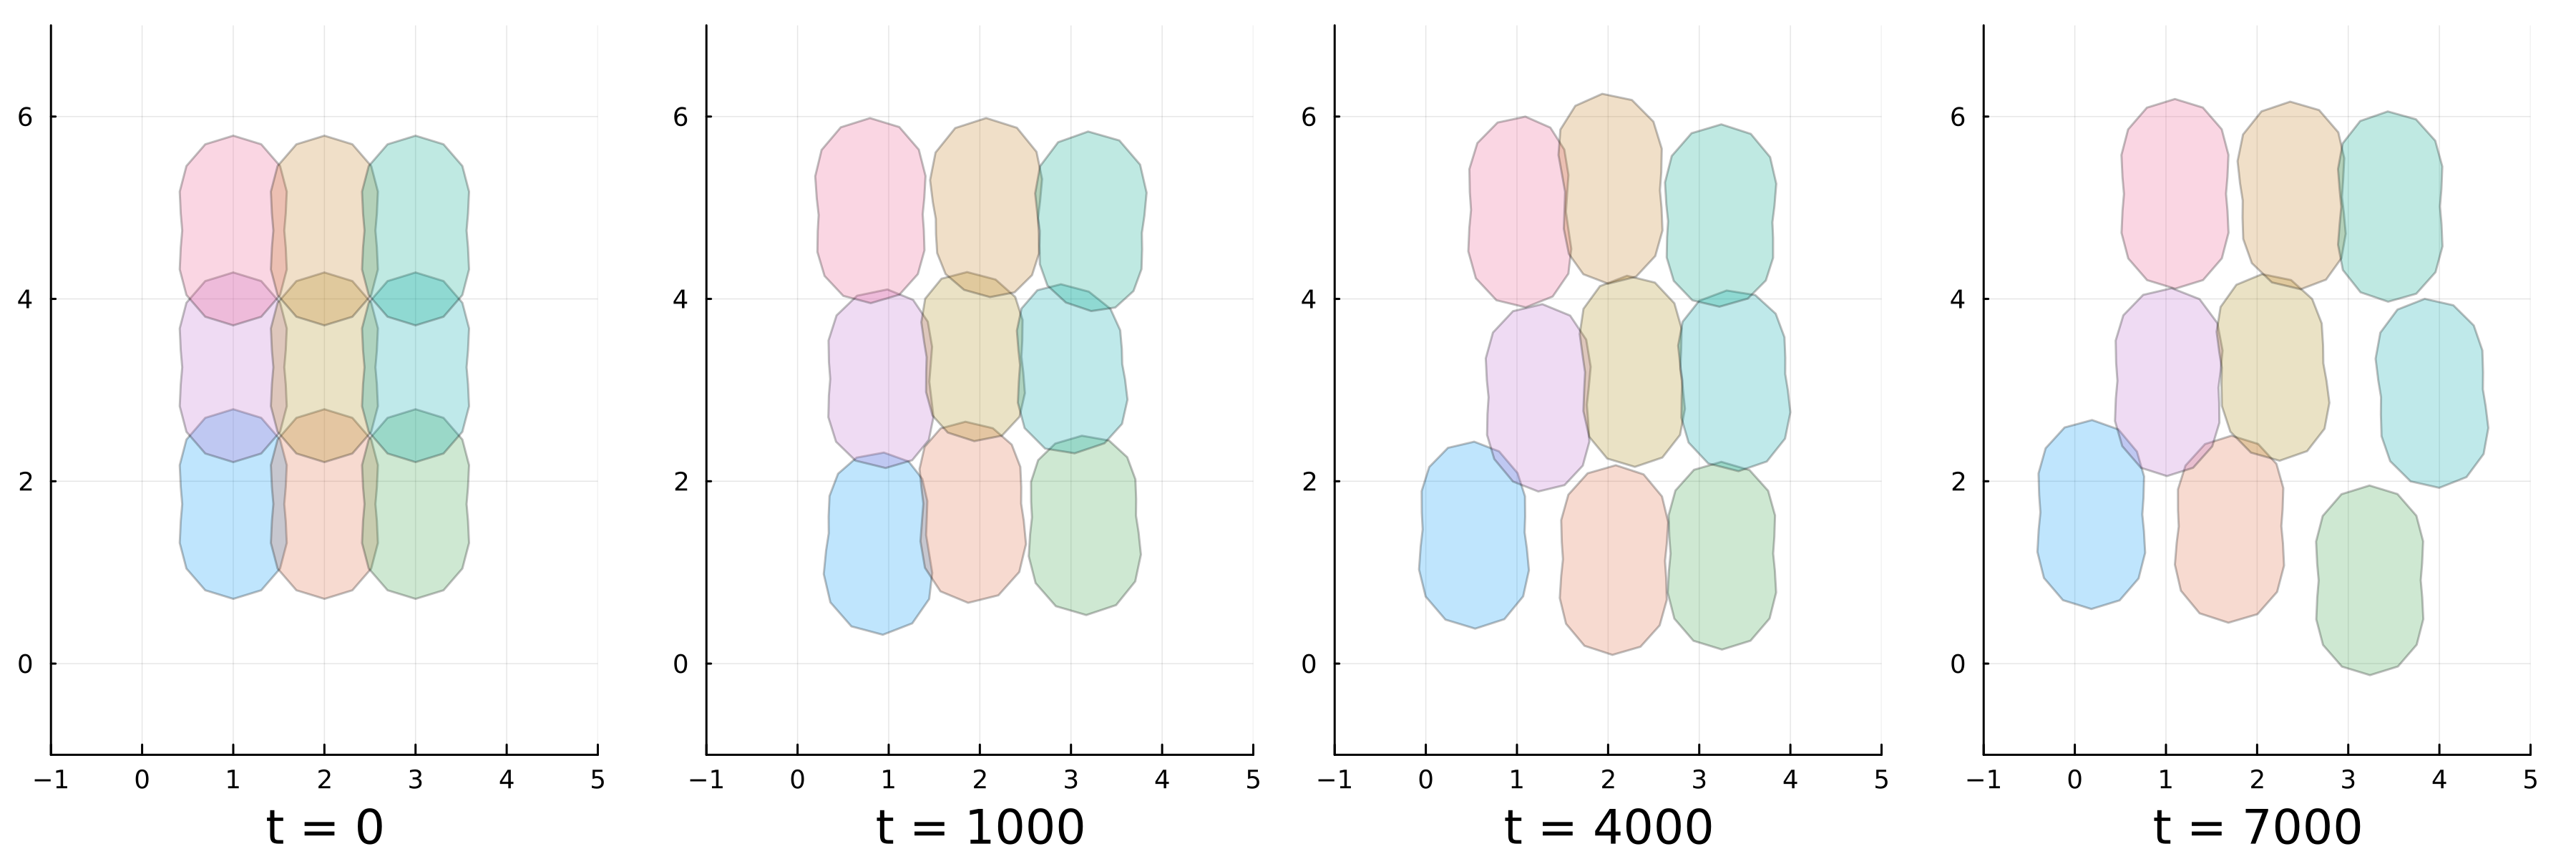
\includegraphics[width=15cm]{bachelors-thesis/forces/interaction/interaction_rescaled/interaction_rescaled.png}
		\caption{This figure shows different plots of a solution to the explained SDE \eqref{eq:interaction2} with the rescaled force configuration. We can see the cells at the times $t \in \{ 0, 1000, 4000, 7000\}$. }
		\label{fig:interaction_rescaled}
	\end{center}
\end{figure}

The \textbf{result of the bachelor's thesis} is a serviceable dynamic with interactions of an entire cellular system.

\newpage
\subsection*{Outlook of bachelor's thesis}
In \cite{Bruna2023} Bruna, Chapman and Schmidtchen studied a macroscopic model for Brownian hard needles. Similar to the hard sphere model in the paper \cite{Bruna2012} from the introduction, there are exclusion effects for the different needle particles. The authors managed to derive an effective PDE that describes the probability density $\rho(t,\vec{x}, \theta)$ of finding a needle with rotation $\theta$ at position $\vec{x}$ and time $t$. An interesting next step for the development of the theory in this thesis would be to derive an effective PDE for our energy dynamic model of the DF cells. \\
